\chapter{Implementation}
\label{chapter:implemntation}

This chapter details the practical development and testing of the system. It
focuses on the integration of various hardware and software components, the
novel modifications made to existing projects, and the challenges encountered
along the way. The discussion covers the connection setup between the Wii Remote
and Raspberry Pi, the streaming of audiovisual data, the extension of Wii Remote
emulation, and the creation of a Python-based input relay.

\section{Establishing Wii Remote Connectivity}
\subsection{Linux Driver Configuration}

One of the initial challenges was to reliably connect the Wii Remote to the
Raspberry Pis. The first step to allow a Wiimote to connect to a Linux machine
is enabling the Linux driver for Wiimotes using the following command:

\begin{lstlisting}[language=bash, emph={modprobe}, emphstyle={\color{magenta}}]
modprobe hid-wiimote
\end{lstlisting}

Running the following command ensures that this driver loads automatically at boot:

\begin{lstlisting}[language=bash]
echo hid-wiimote | sudo tee /etc/modules-load.d/wiimote.conf
\end{lstlisting}

The automated device setup script incorporates this step to ensure that the driver is always loaded correctly.

\subsection{Bluetooth Pairing and Connection}

The next step is to pair the Wii Remote with the Raspberry Pi via Bluetooth. As
Bluetooth requires authorisation to connect two wireless peers, simply loading
the kernel driver is not enough. The Wiimote needs to associate with the Wiimote
with the client machine by trusting it and then establish a connection.

Using the \texttt{bluetoothctl}\cite{bluetoothctl} command-line tool, to pair the Wii Remote with the Raspberry Pi, follow these steps:

\begin{enumerate}
	\item Run \texttt{bluetoothctl} to enter the Bluetooth control interface.
	\item Enter \texttt{scan on} to start scanning for Bluetooth devices.
	\item Immediately press the \textbf{1} and \textbf{2} buttons simultaneously on the Wii Remote to put it in pairing mode.
	\item In the list of discovered bluetooth devices, find the Wii Remote and note its MAC address.
	\item Put the Wii Remote into pairing mode and enter
	      \begin{verbatim}
trust <Wii Remote MAC address>

\end{verbatim}
	      to trust the Wii Remote.

	\item Put the Wii Remote into pairing mode and enter
	      \begin{verbatim}
connect <Wii Remote MAC address>
\end{verbatim}
	      to establish a connection.

\end{enumerate}

If the connection is successful, one of the indicator LEDs on the Wii Remote will remain lit. The Wii Remote is now connected to the Raspberry Pi and ready for use.

\section{Selection of Wii Remote Libraries and Addressing Bluetooth Issues}

Evaluation of multiple libraries and tools for Wii Remote interfacing led to the selection of the xwiimote\cite{xwiimote} library,, particularly for its Python
bindings\cite{xwiimote_bindings}, which allowed for seamless integration into a
Python script. During testing, an issue arose where the Wii Remote connected via
Bluetooth but exhibited continuously flashing lights, with xwiimote failing to
register inputs. Luckily this is a known issue\cite{xwiimote_issue} -- modifying
the Bluetooth configuration file at \texttt{/etc/bluetooth/input.conf} and
adding the following line resolves this issue:

\begin{lstlisting}[language=bash]
ClassicBondedOnly=false
\end{lstlisting}

% # Limit HID connections to bonded devices
% # The HID Profile does not specify that devices must be bonded, however some
% # platforms may want to make sure that input connections only come from bonded
% # device connections. Several older mice have been known for not supporting
% # pairing/encryption.

This setting, when set to \texttt{true}, restricts HID connections to bonded devices only. A bonded device is one that pairs with the host Bluetooth device using a link key, which is a shared secret between the two devices. This setting is useful for ensuring that only trusted devices can connect to the host Bluetooth machine. However, the Wii Remote does not support link key based encryption, so it is necessary to set this value to \texttt{false} to allow the Wii Remote to connect to the client machine. The setup script automates this configuration step to ensure consistent performance across devices.

\section{Audio and Video Streaming Optimisation}
\label{sec:audio-video-streaming}
Streaming audio and video from the host machine to the client machine posed a
significant challenge, with a trade-off observed between media quality and
latency. Higher quality streams resulted in high latency, while lower quality
streams compromised user experience. The solution was to adopt the Real-time
Transport Protocol (RTP) with carefully tuned broadcast and playback settings supported by FFmpeg\cite{wikipediaFFmpeg}. Although further optimisations remain possible, this configuration currently
offers a balanced compromise between low latency and acceptable media quality.

\subsection{\texttt{broadcast-rtp.sh} Script}

The broadcast-rtp.sh script leverages FFmpeg to capture video from the connected
camera device (\texttt{/dev/video0}), encode it in real time, and broadcast it
over the Real-time Transport Protocol (RTP).

The \texttt{broadcast-rtp.sh} script runs the following command:

\begin{lstlisting}[language=bash]
  ffmpeg -max_delay 0 -max_probe_packets 1 -f v412 -framerate 25 -video_size 720x576 -threads 1 -i /dev/video0 -vcodec libx264 -pix_fmt:v yuv420p -g:v 1 -preset ultrafast -tune zerolatency -crf 17 -max_delay 0 -fflags +nobuffer -flags low_delay -f rtp -muxdelay 0 rtp://192.168.20.20:42423
\end{lstlisting}

Table~\ref{tab:broadcast-args} explains the arguments used in the script in detail. See the official \texttt{ffmpeg} documentation for more information\cite{ffmpegDocumentation}. Notably, the script uses the \texttt{-preset ultrafast} option to minimise processing time and the \linebreak \texttt{-tune zerolatency} option to optimise the encoder for real-time transmission which reduces latency. It also uses the \texttt{-crf 17} option which sets the constant rate factor to 17. Constant rate factor (CRF) is a quality-based variable bitrate control method that adjusts the quality of the video stream while maintaining a constant bitrate. In the H.264 codec, the range of the CRF scale is 0–51, where 0 is lossless, 23 is the default, and 51 is worst quality possible. A lower value generally leads to higher quality. A CRF value of 17 or 18 is essentially visually lossless or nearly so\cite{ffmpegEncodeH264x2013}. Keeping the default CRF value of 23, along with the other latency reducing settings, results in video quality that is not acceptable as text and detail become illegible so to increase the quality, the system uses a CRF value of 17.

\begin{table}[!ht]
	\centering
	\begin{tabular}{|p{5cm}|p{10cm}|}
		\hline
		Argument                                        & Explanation                                                                                                          \\ \hline
		`-max\_delay 0`                                 & Processes incoming packets immediately without waiting for additional data, reducing buffering delay.                \\ \hline
		`-max\_probe\_packets 1`                        & Limits probing to one packet to accelerate stream setup.                                                             \\ \hline
		`-f v412`                                       & Specifies the input format provided by the video capture device; ensures compatibility with the incoming video data. \\ \hline
		`-framerate 25`                                 & Sets the frame rate to 25 fps to balance smooth playback and processing load.                                        \\ \hline
		`-video\_size 720x576`                          & Defines the video resolution at 720x576 pixels.                                                                      \\ \hline
		`-threads 1`                                    & Restricts encoding to a single thread for consistent low-latency performance.                                        \\ \hline
		`-i /dev/video0`                                & Specifies the video capture device as /dev/video0.                                                                   \\ \hline
		`-vcodec libx264`                               & Uses the H.264 encoder (libx264) for video encoding.                                                                 \\ \hline
		`-pix\_fmt:v yuv420p`                           & Enforces the yuv420p pixel format for wide compatibility with RTP receivers.                                         \\ \hline
		`-g:v 1`                                        & Forces every frame to be a keyframe, which improves stream recovery and reduces latency.                             \\ \hline
		`-preset ultrafast`                             & Minimises processing time by using the fastest encoding preset.                                                      \\ \hline
		`-tune zerolatency`                             & Optimises the encoder for real-time transmission by reducing latency.                                                \\ \hline
		`-crf 17`                                       & Sets the constant rate factor to balance quality and compression efficiency.                                         \\ \hline
		`-fflags +nobuffer`                             & Disables internal buffering in ffmpeg to minimise latency.                                                           \\ \hline
		`-flags low\_delay`                             & Enables low-delay processing modes for reduced end-to-end latency.                                                   \\ \hline
		`-f rtp`                                        & Specifies the output format as RTP.                                                                                  \\ \hline
		`-muxdelay 0`                                   & Sets the multiplexing delay to zero, ensuring immediate packetisation of the stream.                                 \\ \hline
		`Output Destination: rtp://192.168.20.20:42423` & Designates the target IP address and port for the RTP stream transmission.                                           \\ \hline
	\end{tabular}
	\caption{\texttt{broadcast-rtp.sh} Argument Explanations}
	\label{tab:broadcast-args}

\end{table}



\subsection{\texttt{play-rtp.sh} Script}

The \texttt{play-rtp.sh} script is responsible for receiving and playing the RTP
stream on the client machine. The script runs the following command:

\begin{lstlisting}[language=bash]
  ffplay -vcodec h264 -max_delay 0 -analyzeduration 1 -protocol_whitelist file,udp,rtp -fflags nobuffer -strict experimental -framedrop -flags low_delay -probesize 32 -vf setpts=0 -sync ext rtp-h264.sdp
 \end{lstlisting}

Table~\ref{tab:play-args} explains the arguments used in the script in detail.
See the official \texttt{ffplay} documentation for more
information\cite{ffplayDocumentation}. Notably, the script uses the
\texttt{-sync ext} option to synchronise playback using an external clock,
ensuring accurate timing with the incoming RTP stream. The combination of the
\texttt{-framedrop}, \texttt{-flags low\_delay}, \texttt{-max\_delay 0}, and
\texttt{-fflags nobuffer} options \linebreak helps maintain real-time playback by dropping
frames if necessary, minimising buffering delays, and enforcing low-delay
processing.

\begin{table}[!ht]
	\centering
	\begin{tabular}{|p{5cm}|p{10cm}|}
		\hline
		Argument                            & Explanation                                                                                                             \\ \hline
		`-vcodec h264`                      & Specifies that the incoming stream is encoded in H.264, ensuring the correct decoder is used.                           \\ \hline
		`-max\_delay 0`                     & Eliminates buffering delays on the playback side, promoting real-time viewing.                                          \\ \hline
		`-analyzeduration 1`                & Limits the analysis duration to speed up the startup process.                                                           \\ \hline
		`-protocol\_whitelist file,udp,rtp` & Whitelists required protocols (file, UDP, RTP) for reading the SDP file and handling the RTP stream.                    \\ \hline
		`-fflags nobuffer`                  & Disables input buffering to reduce latency during playback.                                                             \\ \hline
		`-strict experimental`              & Allows usage of experimental features if necessary for stream compatibility.                                            \\ \hline
		`-framedrop`                        & Drops frames if decoding lags, keeping playback as close to real-time as possible.                                      \\ \hline
		`-flags low\_delay`                 & Enforces low-delay processing to maintain alignment with the low-latency broadcast.                                     \\ \hline
		`-probesize 32`                     & Sets a minimal data probe size (32 bytes) to reduce initialisation time.                                                \\ \hline
		`-vf setpts=0`                      & Resets presentation timestamps to help maintain sync in a low-latency context.                                          \\ \hline
		`-sync ext`                         & Synchronises playback using an external clock for accurate timing with the RTP stream.                                  \\ \hline
		`Input File: rtp-h264.sdp`          & Provides the SDP file that describes the RTP stream parameters, essential for interpreting the incoming data correctly. \\ \hline
	\end{tabular}
	\caption{\texttt{play-rtp.sh} Argument Explanations}
	\label{tab:play-args}

\end{table}




\section{Python Script for Input Relay}
A core component of the project is the custom Python script
(\texttt{input\_relay.py}) that serves as a bridge between the physical
Wii Remote and the emulation backend running on the host Raspberry Pi. This
script leverages the \texttt{xwiimote} Python bindings to interface directly
with the Wii Remote hardware, continuously monitoring for various input events
and relaying them to the Wii Remote Emulator via UDP.

\subsection{Wiimote Connection and Monitoring:}
The script initialises a \texttt{xwiimote} monitor to detect when a Wii Remote connects to the client machine. When the input relay detects a device, it creates an interface with the device and opens it for both reading and writing. This method of setting up the Wii Remote connection differs from the traditional approach other libraries use, which typically use the device files located in the \texttt{\\dev} directory automatically without the need for manual setup.

\subsection{Non-Blocking I/O and Event Polling:}
Using the \texttt{select.poll()} mechanism, the script sets up non-blocking I/O on the Wii Remote’s file descriptor. This allows the script to efficiently wait for input events without stalling the main event loop. When the script detects events, the script calls \texttt{dev.dispatch(evt)} to process them.

\subsection{Event Processing and Binary Packet Formation:}
Depending on the event type, the script processes the data accordingly:

\subsubsection{Accelerometer Events}
When the machine receives an accelerometer event (identified by \linebreak \texttt{xwiimote.EVENT\_ACCEL}), the script retrieves the raw accelerometer values from channel 0. It then normalises these values (using a custom scaling and offset transformation) and packs them into a binary packet with the header \texttt{0x02}. The binary format is:
\begin{center}
	\texttt{[1 byte event type (0x02)] + [4 bytes float ax] +}
	\texttt{[4 bytes float ay] + [4 bytes float az]}
\end{center}

\subsubsection{IR Events:}
For IR events (identified by \texttt{xwiimote.EVENT\_IR}), the script retrieves the IR coordinates and normalises them to a [0,1] range. It then packs the data into a binary packet with header \texttt{0x01}:
\begin{center}
	\texttt{[1 byte event type (0x01)] + [4 bytes float x] +}
	\texttt{[4 bytes float y] + [4 bytes float z]}
\end{center}

\subsubsection{Button (Key) Events:}
The script also processes key events (e.g., pressing the \texttt{+}, \texttt{HOME}, \texttt{A}, etc buttons). For context, Figure~\ref{fig:wiimote_buttons} shows the layout of the Wii Remote buttons. The input relay handles these by sending text-based command packets (e.g., \texttt{"button 1 WIIMOTE\_PLUS"}) over UDP to indicate button press and release actions.

\begin{figure}[h]
	\centering
	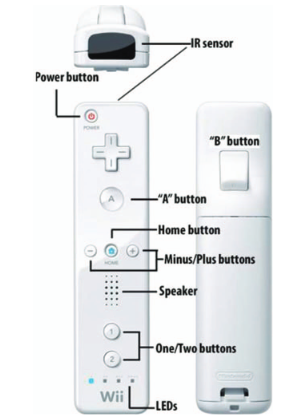
\includegraphics[width=0.6\textwidth]{wii_remote.png}
	\caption{Wii Remote Button Layout. Image source\cite{wiimoteButtons}}
	\label{fig:wiimote_buttons}
\end{figure}


\subsection{UDP Communication:}
The script creates a UDP socket to transmit the binary (and text-based) update packets to the Wii Remote Emulator. The user provides the IP address and port of the host machine running the Wii Remote emulator via command-line arguments. The script logs key actions and any errors using Python’s built-in logging facilities, ensuring that debugging information is available during operation.

\subsection{Robust Error Handling:}
The script catches and logs exceptions (such as I/O errors during event dispatching). This approach ensures that transient errors do not break the event loop, thereby maintaining reliable real-time transmission of control data while providing feedback to the user. The script also handles keyboard interrupts gracefully, ensuring that the Wii Remote connection is properly closed before exiting.

\section{Wii Remote Emulation Enhancements}

The system’s final major component is the emulation of the Wii Remote on the host
Raspberry Pi. The implementation utilises a modified version of the
\texttt{WiimoteEmulator} originally developed by Ryan
Conrad\cite{wiimote_emulator} (known as rnconrad on GitHub).
\texttt{WiimoteEmulator} is able to emulate a Bluetooth Wii controller in
software, enabling control of the Wii through various different input devices such
as a keyboard, mouse, or text commands over a network.

More specifically, this project builds on a fork of the project by
JRogaishio\cite{jr_wiimote_emu} as it fixes two critical bugs. The first bug is
that the IP command in the original project was not working due to an index
error. The second bug is that the original project was not compiling due to a
call to \texttt{graceful\_disconnect()} which was not defined.

The version created in this project\cite{kf_wiimote_emu} builds upon this fork by adding support for transmitting IR and accelerometer data through the IP socket interface.

\subsection{Enhancements}


\subsubsection{IR Emulation}

IR emulation in the system is responsible for generating the infrared (IR)
sensor data that the Wii Remote expects when pointing at a sensor bar. The
implementation leverages the functions defined in \texttt{motion.c}. First, the
function \linebreak \texttt{look\_at\_pointer} computes a transformation matrix based on
normalised pointer coordinates (\texttt{pointer\_x} and \texttt{pointer\_y}).
This matrix defines the orientation of the emulated Wii Remote relative to a
virtual screen, factoring in physical dimensions (e.g., screen width, sensor bar
width) and viewing distance.

Next, \texttt{set\_motion\_state} uses this transformation to compute two sensor
points (\texttt{sensor\_pt0} and \texttt{sensor\_pt1}). In this process, a sensor point is defined as
\[
p = (p_x, p_y, p_z, p_w)
\]


A custom perspective projection matrix (\texttt{make\_cam\_projection\_mat}) projects these points into a normalised coordinate system. Putting a sensor point through this perspective divide and normalisation yields:

\[
p' = \left(\frac{p_x}{p_w},\, \frac{p_y}{p_w},\, \frac{p_z}{p_w}\right).
\]

The normalised coordinates are then mapped to screen space and used to compute the IR sensor output as follows:
\[
\begin{aligned}
x_{\text{ir}} &= \text{round}\!\Bigl(1023 \cdot \frac{p'_x + 1}{2}\Bigr),\\[1mm]
y_{\text{ir}} &= \text{round}\!\Bigl(767 \cdot \frac{p'_y + 1}{2}\Bigr),\\[1mm]
\text{size} &= \text{round}\!\Bigl(\text{min\_pt\_size} + \Bigl(1 - p'_z\Bigr)^2 \cdot \bigl(\text{max\_pt\_size} - \text{min\_pt\_size}\bigr)\Bigr),
\end{aligned}
\]
with \(\text{min\_pt\_size} = 1.0\) and \(\text{max\_pt\_size} = 15.0\).

This process ensures that the emulated IR data closely mimics the signals produced by a real Wii Remote when pointing at a sensor bar.


\subsubsection{Accelerometer Emulation}

Accurately emulating the Wii Remote accelerometer involves reading accelerometer data transmitted from the client machine over the network, processing this data, and effectively injecting it into the emulated Wii Remote state on the host machine. This component is critical for games that heavily rely on motion controls, such as racing and sports games, which interpret device orientation and motion through accelerometer inputs.

The Wii Remote Emulator captures the binary accelerometer packets using a non-blocking UDP socket interface implemented in \texttt{input\_socket.c}. Upon receiving a packet, the emulator extracts the floating-point acceleration values using a network-to-host float conversion function \texttt{ntohf()}. Specifically, the following procedure occurs within the emulator's UDP socket polling loop:

\begin{enumerate}
	\item Check if the packet starts with the correct identifier byte (\texttt{0x02}) and has the correct packet size (13 bytes).
	\item Extract the network-order binary floats representing accelerations along the three axes.
	\item Convert these network-order floats to host-order floats using \texttt{ntohf()}.
\end{enumerate}

These extracted values are then assigned directly into the Wii Remote emulator’s state structure:

\begin{lstlisting}[language=C]
state->usr.accel_x = event.analog_motion_event.x;
state->usr.accel_y = event.analog_motion_event.y;
state->usr.accel_z = event.analog_motion_event.z;
\end{lstlisting}

The input relay normalises the raw accelerometer data before transmitting it to the emulator. Thus, the Wii Remote emulator can directly use these values to update the emulated Wii Remote’s accelerometer state.

\subsubsection{Latency Reduction}

Latency is a critical performance metric when determining the playability of video games. In general, the lower the latency, the more responsive the game feels to the player. As such, minimising latency across the system was a key focus during development. The system employs several strategies to reduce latency and improve responsiveness, including:

\begin{itemize}
	\item \textbf{Non-blocking I/O:} In the \texttt{input\_socket.c} file, UDP
	      sockets use the \linebreak \texttt{SOCK\_NONBLOCK} flag to ensure that the system
	      can continuously poll for new input events without stalling on network reads.
	      Without this flag, the emulator would block on network reads meaning that the
	      emulator would not be able to process any other events until the network read is
	      complete. This is especially important since the input relay is streaming the IR
	      and accelerometer data to the emulator in close to real-time so the emulator
	      could miss multiple events if it was blocking on reads.
	\item \textbf{Optimised Data Pipelines:} The system uses lightweight binary
	      protocols for both IR and accelerometer updates. Sending fixed-length packets
	      (e.g., 13-byte packets for IR and accelerometer data) reduces the overhead associated
	      with parsing, improving overall throughput.

\end{itemize}

A shown in the \nameref{sec:playability-analysis}, the latency introduced by the emulator is minimal, with the majority of latency stemming from the video streaming component.

\section{Automation of Device Setup}

To streamline the deployment process, the project includes a device setup script (\texttt{setup.sh}). This script requires administrative privileges (sudo) and automates several critical configuration tasks, including:

\begin{itemize}

	\item Loading necessary kernel modules.
	\item Editing system files (such as /etc/bluetooth/input.conf) to adjust Bluetooth settings.
	\item Configuring environment variables and export paths for library dependencies.
	\item Installing \texttt{xwiimote} and its Python bindings.
	\item Downloading and compiling the custom Wii Remote Emulator.
\end{itemize}

By automating these tasks, the setup script minimises manual configuration errors and ensures a consistent environment across multiple devices.

%% \section{Testing and Validation}
%% Rigorous testing was conducted to evaluate the performance and reliability of the system

%% \subsubsection{Connectivity Tests}
%% Confirmed that the Wii Remote establishes a stable connection with the Raspberry Pis under various conditions.

%% \subsubsection{Latency and Quality Measurements}
%% Evaluated the balance between media quality and streaming latency, with iterative tuning of RTP settings.

%% \subsubsection{End-to-End Gameplay Trials}
%% Real-world testing using games such as Mario Kart provided insights into the system’s responsiveness and highlighted areas for future refinement, particularly regarding latency and IR display limitations.







% First challenge was getting the wii remote to connect to the raspberry pis. Required enabling the wii remote Linux drivers using 'modprobe hid-wiimote'. To ensure this always gets loaded at boot time, add it to the modules-load.d configuration: 'echo hid-wiimote | sudo tee /etc/modules-load.d/wiimote.conf'.
%
% Many different wiimote libraries and tools. Decided to use xwiimote (reference) and more specifically used xwiimote python bindings (reference) to create a python script
%
% Ran into issue where remote would connect through bluetooth but lights would keep flashing and xwiimote could not detect it. Have to edit '/etc/bluetooth/input.conf' and add the line 'ClassicBondedOnly=false'. (reference https://github.com/xwiimote/xwiimote/issues/109)
%
% Another challenge was streaming the audio and video from the host pi to the client pi. Main issue was either quality or latency. Higher quality was causing very high latency and vice versa. Solved by using rtp protocol with some very specific setting (show broadcast and play commands here??)
%
% Another part of the project was doing the wii remote emulation from the host pi to the wii. Used a modified version of Wiimote emulator by rnconrad (reference). Specifically modified JRogaishio's fork (reference) of the project whose changes have yet to merged to the original project. Used this fork as it fixes the ip version of the project which allows for receiving commands over a network which is what I want. Also adds some more documentation and fixes a compilation error. My version (reference) adds support for IR and accelerometer data over the ip socket interface. Many challenges here. Mainly figuring out all the accelerometer and IR maths in motion.c as well as adding all the plumbing in input.c and input_socket.c.
%
% Also latency issues which have not been resolved. Also issue with IR not going above bottom half of the screen. Potential issue of the tuning of accelerometer will be mario kart specific

% Last hard part was creating the python script that takes all the real wiimote inputs and translates then sends them to the wiimote emulator on the host pi.
%
% Maybe creating a device setup script that requires sudo and does all the changing of system files, drivers, Export paths for libs, etc
